\documentclass{standalone}
\usepackage{ tikz }
\usepackage{ xparse }
\input{macros/all}

\begin{document}
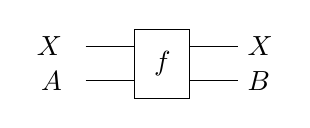
\begin{tikzpicture}[yscale=-1,x=1em,y=1.25em]
        

    \draw (0.5,0.5) -- (2.25,0.5); 
    \draw (0.5,1.5) -- (2.25,1.5);

    \draw (4.25,0.5) -- (6,0.5);
    \draw (4.25,1.5) -- (6,1.5);
    
    \node[draw, minimum height = 2.5em, minimum width = 2em, anchor = west, fill=white] at (2.25,1){$f$};
    \node[anchor = east] at (0,0.5){$X$};
    \node[anchor = east] at (0,1.5){$A$};
    \node[anchor = west] at (6,0.5){$X$};
    \node[anchor = west] at (6,1.5){$B$};

\end{tikzpicture}
\end{document}